\documentclass[a1paper,portrait,american,fontscale=.4]{baposter}

\usepackage{lipsum}
\usepackage{listings}
\usepackage{todo}
\usepackage{hyperref}
\usepackage{qrcode}
\usepackage{tikz}
\usetikzlibrary{
    arrows,
    arrows.meta,
    backgrounds,
    calc,
    chains,
    decorations,
    decorations.pathreplacing,
    matrix,
    positioning,
    scopes,
    shadows,
    shapes,
    shapes.multipart,
}

\definecolor{MyColorOne}{HTML}{637462}
\definecolor{MyColorTwo}{HTML}{b7af8a}
\definecolor{MyColorThree}{HTML}{ccb15a}

\tikzstyle{rect}=[draw,rectangle,thick,on chain,font=\tiny,inner sep=1mm,minimum height=1.25em]

\begin{document}
\begin{poster}{
        %----- Poster Settings -----------------------------------------------------------------------------------------
        background=none,
        columns=5,
        %----- Box Settings --------------------------------------------------------------------------------------------
        boxColorOne=white!96!black,
        %boxColorOne=MyColorTwo!30!white,
        %boxColorTwo=MyColorThree!30!white,
        %boxshade=shadeTB,
        boxshade=plain,
        headershade=shadeLR,
        headerColorOne=MyColorOne,
        headerColorTwo=MyColorTwo,
        textborder=roundedleft,
        borderColor=black,
        headerborder=open,
        headershape=roundedright,
        headerfont=\large\bfseries,
        headerFontColor=white!90!MyColorTwo,
        linewidth=0pt,
    }
    {}
    {
        ACM~SIGMOD'19~Programming~Contest
    }
    {
        \vspace*{.5em}
        \bfseries
        \emph{teamsic:}~Immanuel~L.~Haffner
    }
    {
    }

    \headerbox{Task Description}{name=task,column=0,span=3}{
        \begin{itemize}
            \item 2x Intel Xeon E5-2640v4 @2.4GHz (10 cores, 20 hypterthreads, 25\,MiB cache, AVX-2)
            \item 30\,GiB RAM
            \item Ubuntu 17.10 with Linux 4.13
            \item 2 1.6\,TB SATA-6GBPS SSD (500\,MB/s read, 475\,MB/s write)
        \end{itemize}

        \begin{center}
            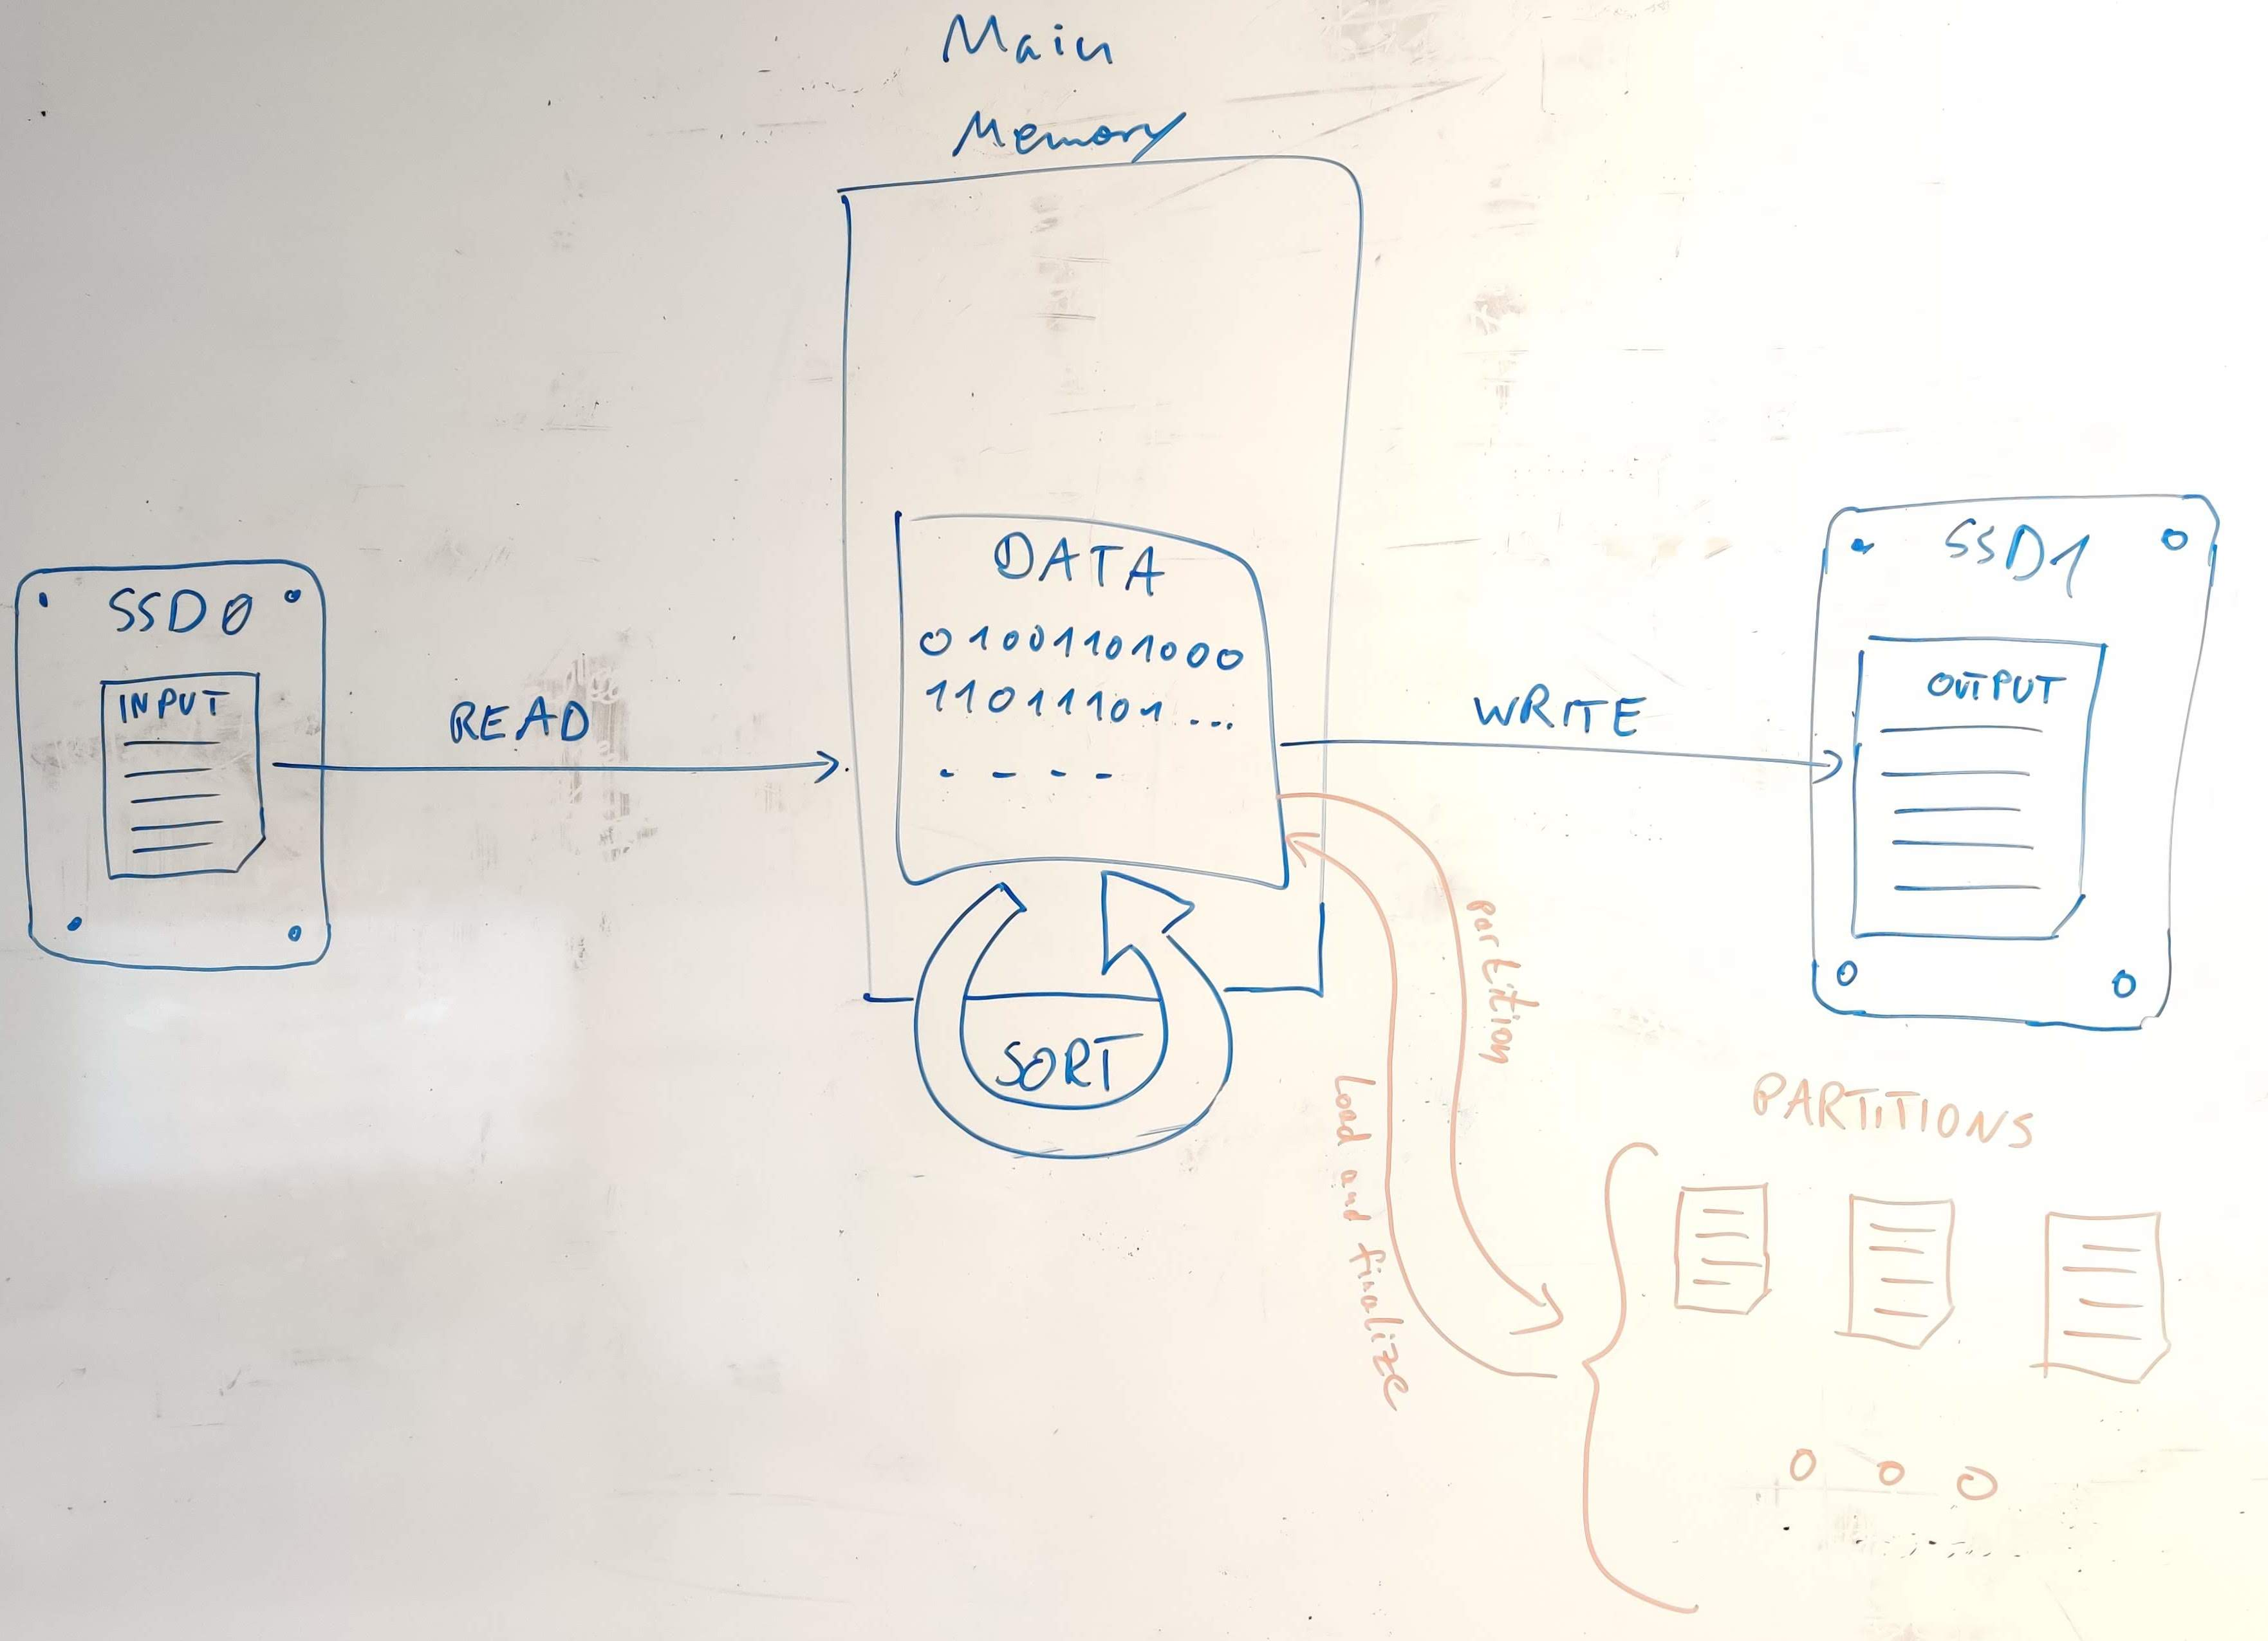
\includegraphics[scale=.25]{fig/task_overview.jpg}
        \end{center}

        \textbf{100\,byte record:}
        \begin{center}
            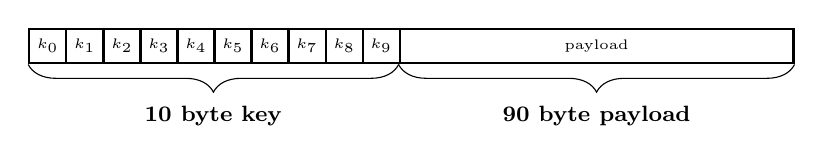
\begin{tikzpicture}
                \begin{scope}[start chain=going right,node distance=-\pgflinewidth]
                    \node[rect] (k0) {$k_0$};
                    \node[rect] {$k_1$};
                    \node[rect] {$k_2$};
                    \node[rect] {$k_3$};
                    \node[rect] {$k_4$};
                    \node[rect] {$k_5$};
                    \node[rect] {$k_6$};
                    \node[rect] {$k_7$};
                    \node[rect] {$k_8$};
                    \node[rect] {$k_9$};
                    \node[rect,minimum width=50mm] (payload) {payload};
                    \draw[decorate,decoration={brace,mirror,amplitude=10pt}]
                    (k0.south west) -- node[below=4mm] {\footnotesize\textbf{10 byte key}} (payload.south west);
                    \draw[decorate,decoration={brace,mirror,amplitude=10pt}]
                    (payload.south west) -- node[below=4mm] {\footnotesize\textbf{90 byte payload}} (payload.south east);
                \end{scope}
            \end{tikzpicture}
        \end{center}

        \begin{itemize}
            \item distinguish between in-memory sorting task and external sorting task
        \end{itemize}
    }

    \headerbox{Sorting Algorithm}{name=algo,column=3,span=2}{
        \begin{itemize}
            \item in-place radix sort with \emph{American Flag Sort}
            \item parallelize on first recursion: use one thread per call (work list) or all threads per call
            \item custom concurrent American Flag Sort partitioning
            \item fall back to \texttt{std::sort()} below certain threshold (i.e.\ \emph{introsort} with fall back to
                \emph{insertion sort})
        \end{itemize}

        \begin{center}
            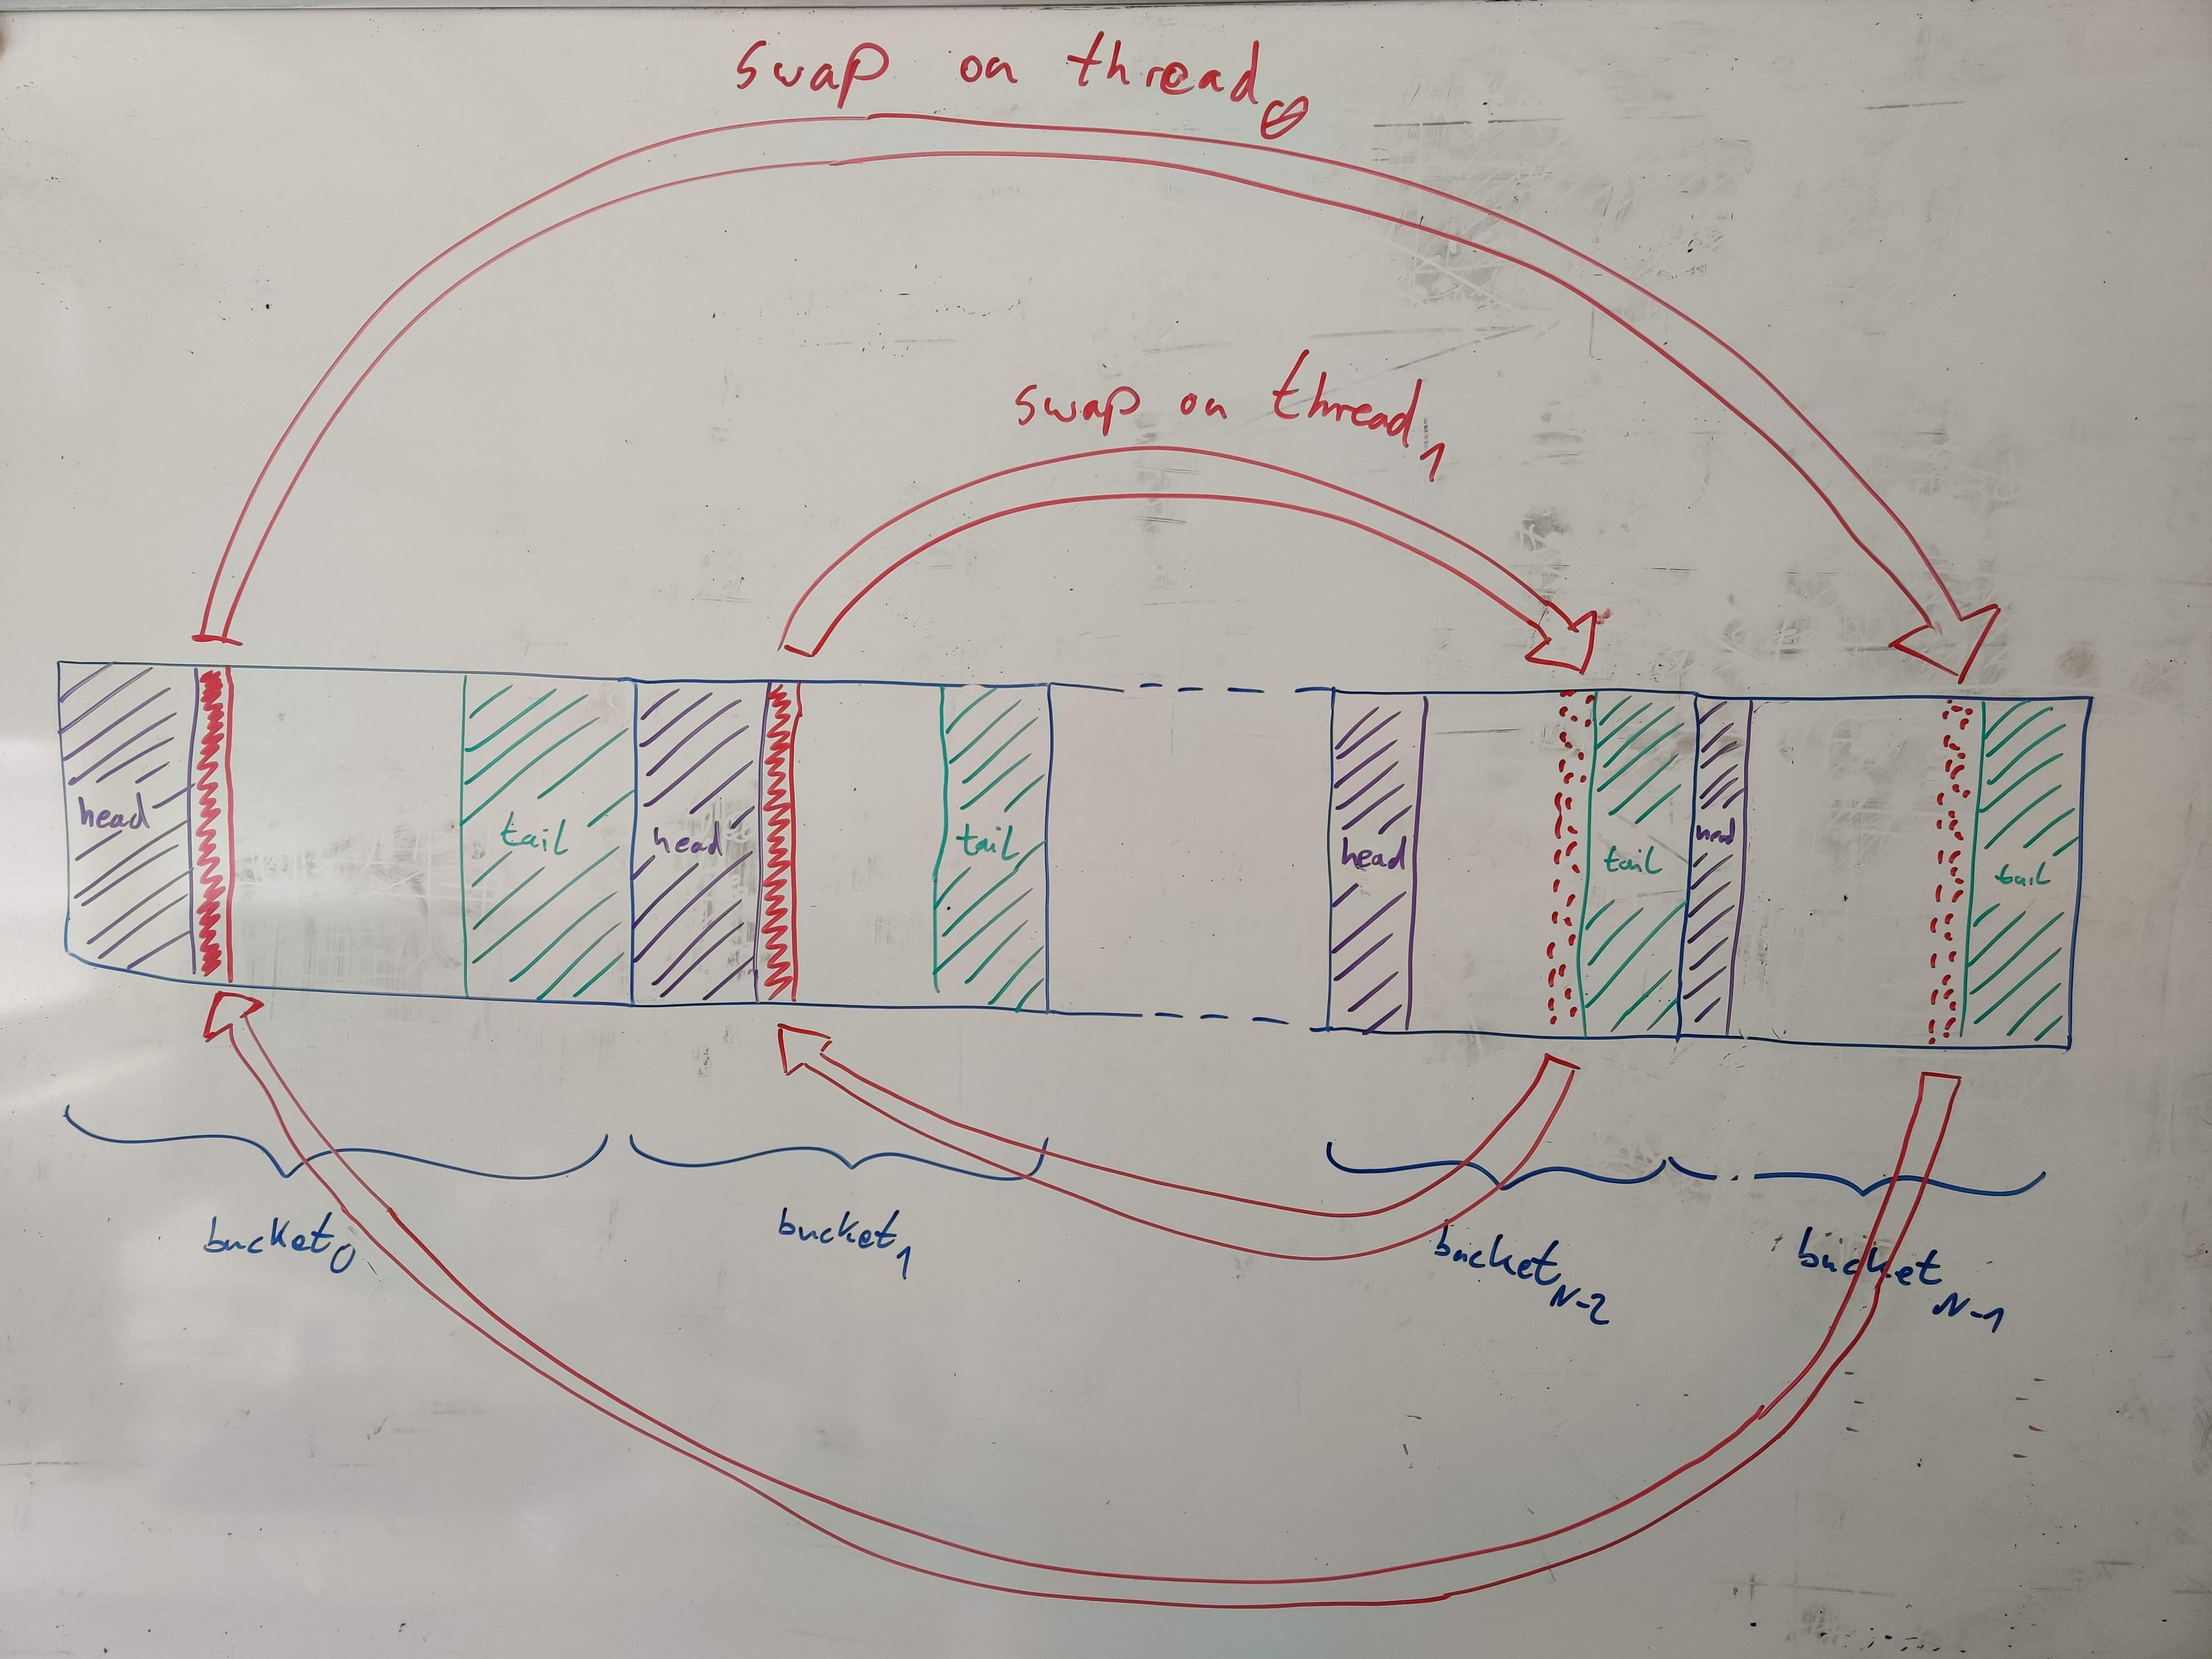
\includegraphics[scale=.05]{fig/parallel_AFS.jpg}
        \end{center}
    }

    \headerbox{In-Memory Sorting}{name=inmemory,column=3,span=2,below=algo}{
        \begin{itemize}
            \item \texttt{mmap()} the entire output file and read the input file into that memory region
            \item decide whether all values $[0 - 255]$ or only printable ASCII $[32-126]$ by inspection of first $10$
                records
            \item assume uniform distribution of keys
            \item already partition on first byte while reading from input file
            \item finish partitions in parallel with American Flag Sort
            \item don't write to disk; terminate the application $\rightarrow$~kernel takes care to write changed
                \texttt{mmap()}'d file back to disk
        \end{itemize}
    }

    \headerbox{External Memory Sorting}{name=external,column=0,span=3,below=task}{
        \begin{itemize}
            \item read as much data as fits into main memory
            \item sort that data with parallel American Flag Sort on NUMA region~0
            \item in parallel, partition remaining data into 256 buckets on SSD1 on NUMA region~1
            \item starting with the smallest bucket, load a bucket, sort it, then merge the bucket with the sorted in
                memory data and write it to the output file on disk
        \end{itemize}

        \begin{center}
            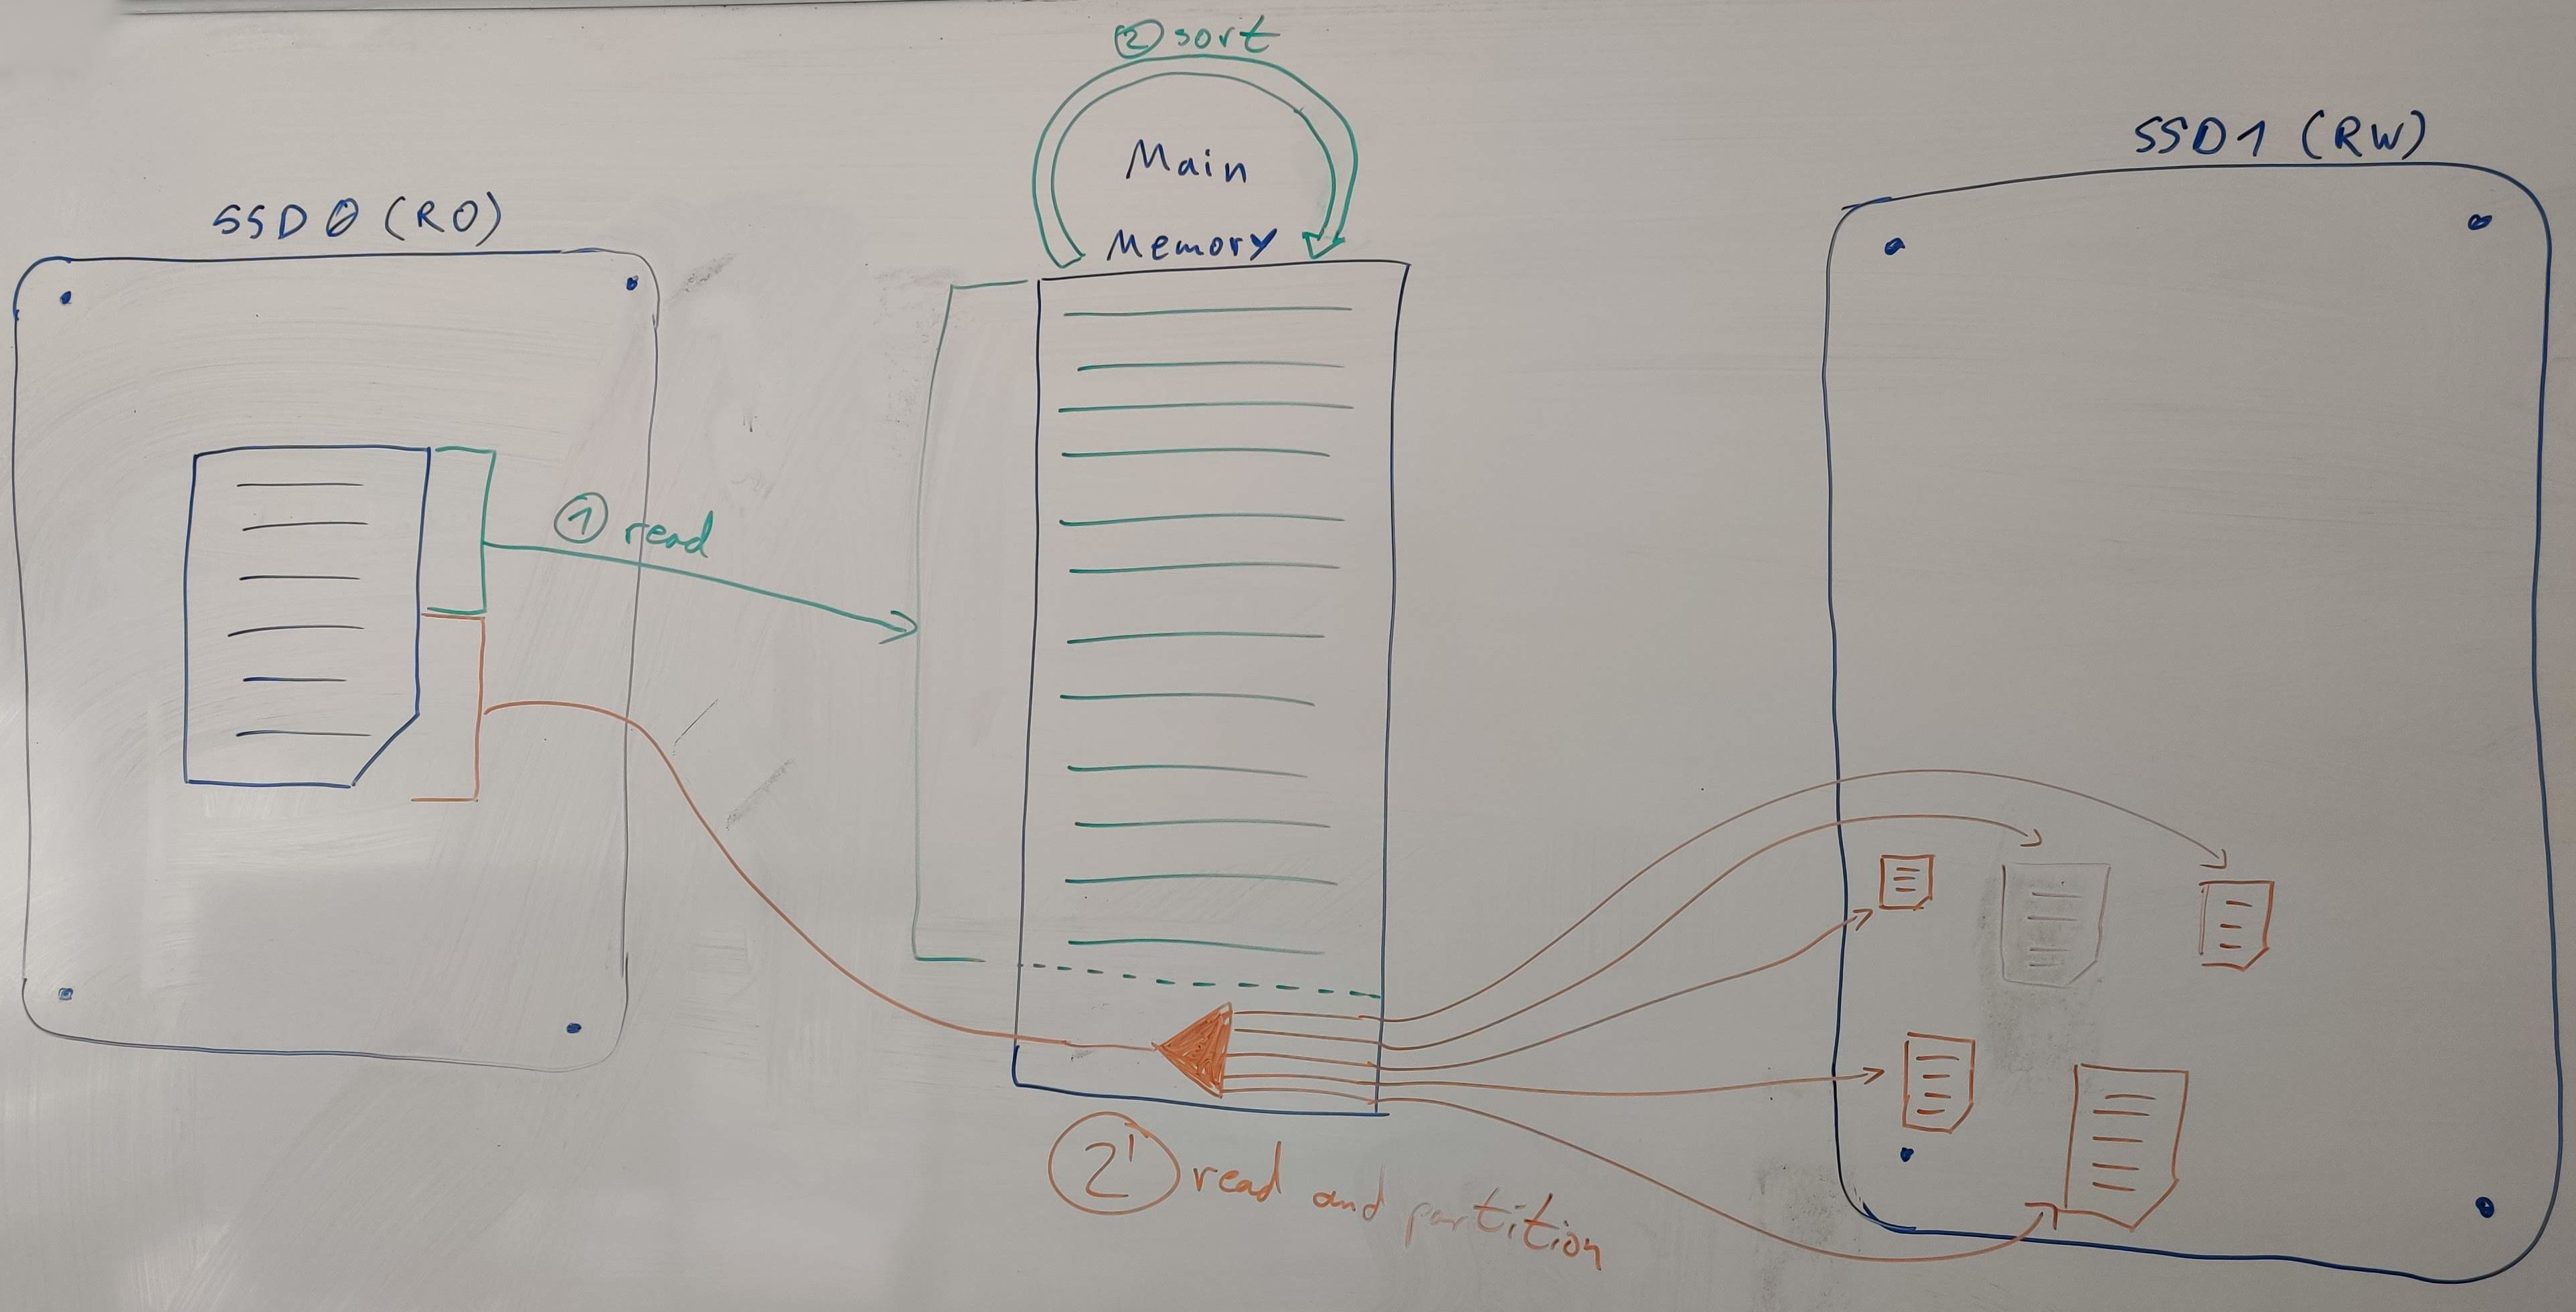
\includegraphics[scale=.2]{fig/external_sort_1.jpg}
            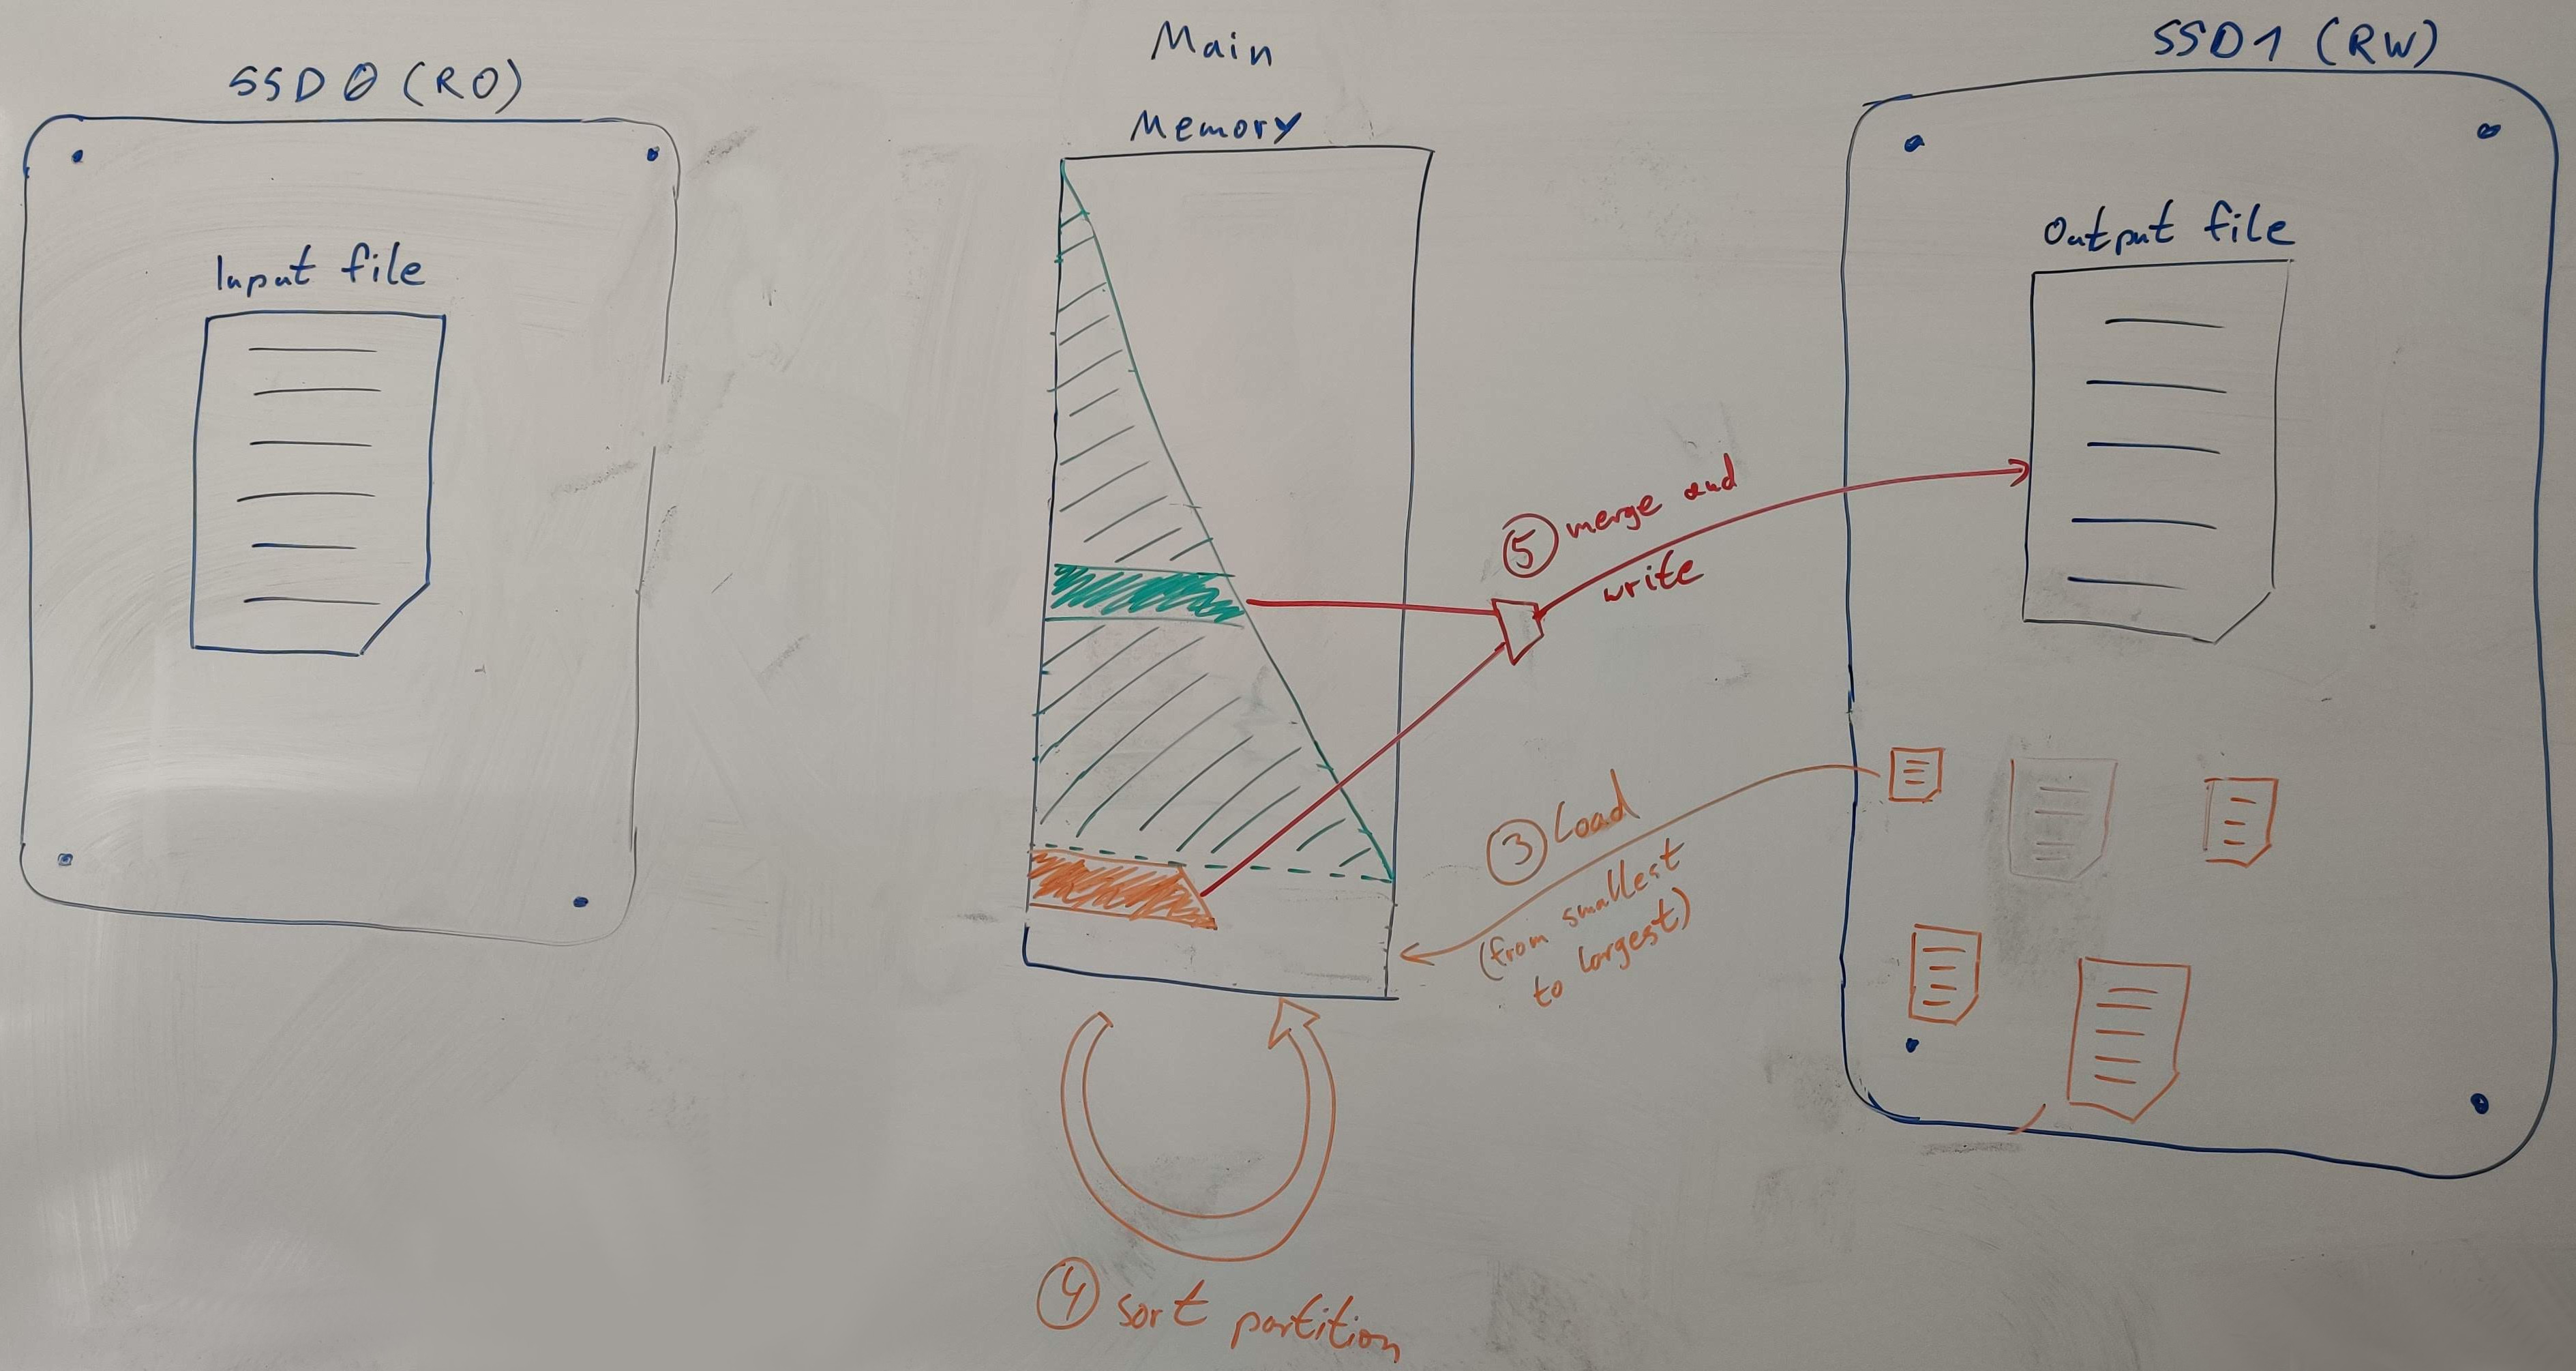
\includegraphics[scale=.2]{fig/external_sort_2.jpg}
        \end{center}

        \begin{minipage}[t][66mm][c]{.53\textwidth}
            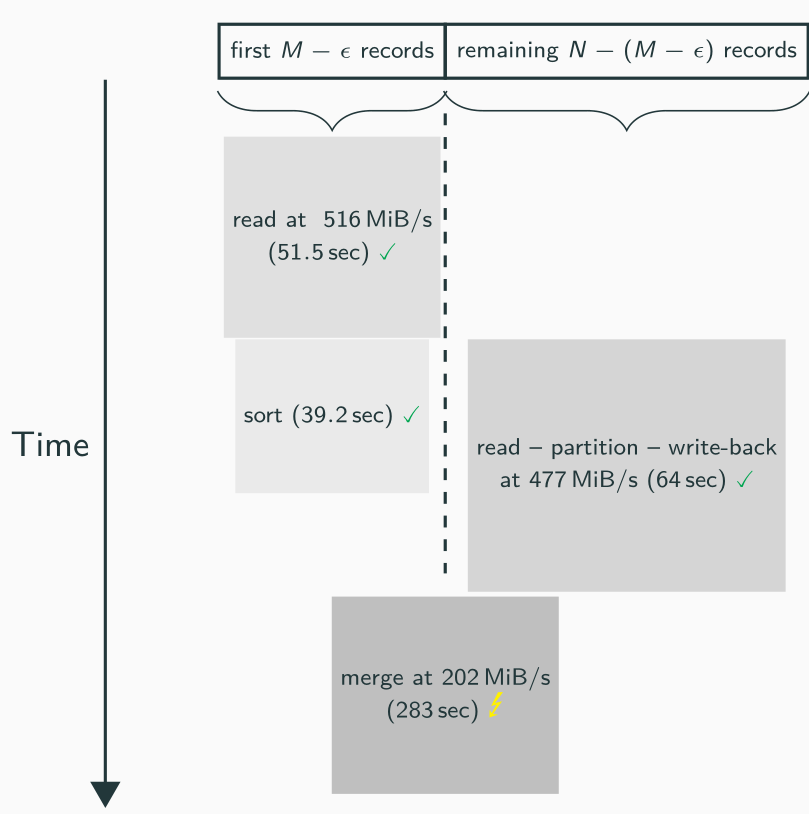
\includegraphics[scale=.18]{fig/timeline.png}
        \end{minipage}%
        \begin{minipage}[t][66mm][c]{.47\textwidth}
            \begin{enumerate}
                \item Read the first $M - \epsilon$ records into main memory.
                \item Start to sort the $M - \epsilon$ records.
                \item[2'.] Concurrently read the remaining $N - (M - \epsilon)$ records and partition them into $256$ buckets
                    on SSD1.

                \item Load the next smallest partition into main memory.
                \item Sort the records in the partition.
                \item Merge the sorted partition with the sorted in-memory data and write to output file on SSD1.
            \end{enumerate}
        \end{minipage}
    }

    \headerbox{Third-Party Libraries}{name=libs,column=3,span=2,below=inmemory}{
        \begin{itemize}
            \item Agner Fog's \texttt{asmlib} {\footnotesize (for \texttt{memcmp()})}
            \item CTPL: Modern and Efficient C\texttt{++} Thread Pool Library {\footnotesize (not in final submission)}
            \item Intel Processor Counter Monitor (PCM) {\footnotesize (not in final submission)}
        \end{itemize}
    }

    \headerbox{Source Code}{name=code,column=3,span=2,below=libs}{
        \begin{minipage}[b]{.65\linewidth}
            The source code is available on Github and licensed under Apache~v2.
        \end{minipage}%
        \begin{minipage}[t]{.35\linewidth}
            \begin{flushright}
                \qrcode[height=22mm]{https://git.io/fjazH}
                \\[.5em]
                \mbox{\url{git.io/fjazH}}
            \end{flushright}
        \end{minipage}
    }
\end{poster}
\vspace*{-6em}
\begin{flushright}
    \footnotesize
    Big~Data~Analytics~Group \\[.5em]
    \url{bigdata.uni-saarland.de} \\[.5em]
    Saarland~Informatics~Campus \\[.5em]
\end{flushright}
\clearpage
\todos
\end{document}
